\documentclass[12pt]{article}
\usepackage[margin = 1in]{geometry}
\usepackage{amsmath}
\usepackage{amssymb}
\usepackage{amsthm}
\usepackage{graphicx}
\usepackage{subfig}
\usepackage{enumitem}

\begin{document}
	
	\begin{center}
		\textbf{Quiz 10} \\
		\textbf{Differential Equations} \\
		\textbf{Math 337} \\
		\textbf{Stephen Giang} \\
	\end{center}

\noindent \textbf{Problem 1: } Consider the function $f(t)$ defined as follows:
	$$
	f(t) = 
	\begin{cases}
		t^2 + 1 & 0 \leq t \leq 3 \\
		0 & t > 3
	\end{cases}
	$$
Sketch a graph of this function and write it in terms of the step function, $u_c(t)$, which is defined in the lecture notes. Further, write the function with the step function so that every element is readily found in the Laplace table. (Something like $u_c(t) \sin(t - c)$.) Finally, find the Laplace Transform of $f(t), F(s) = \mathcal{L}[f(t)]$.
\\
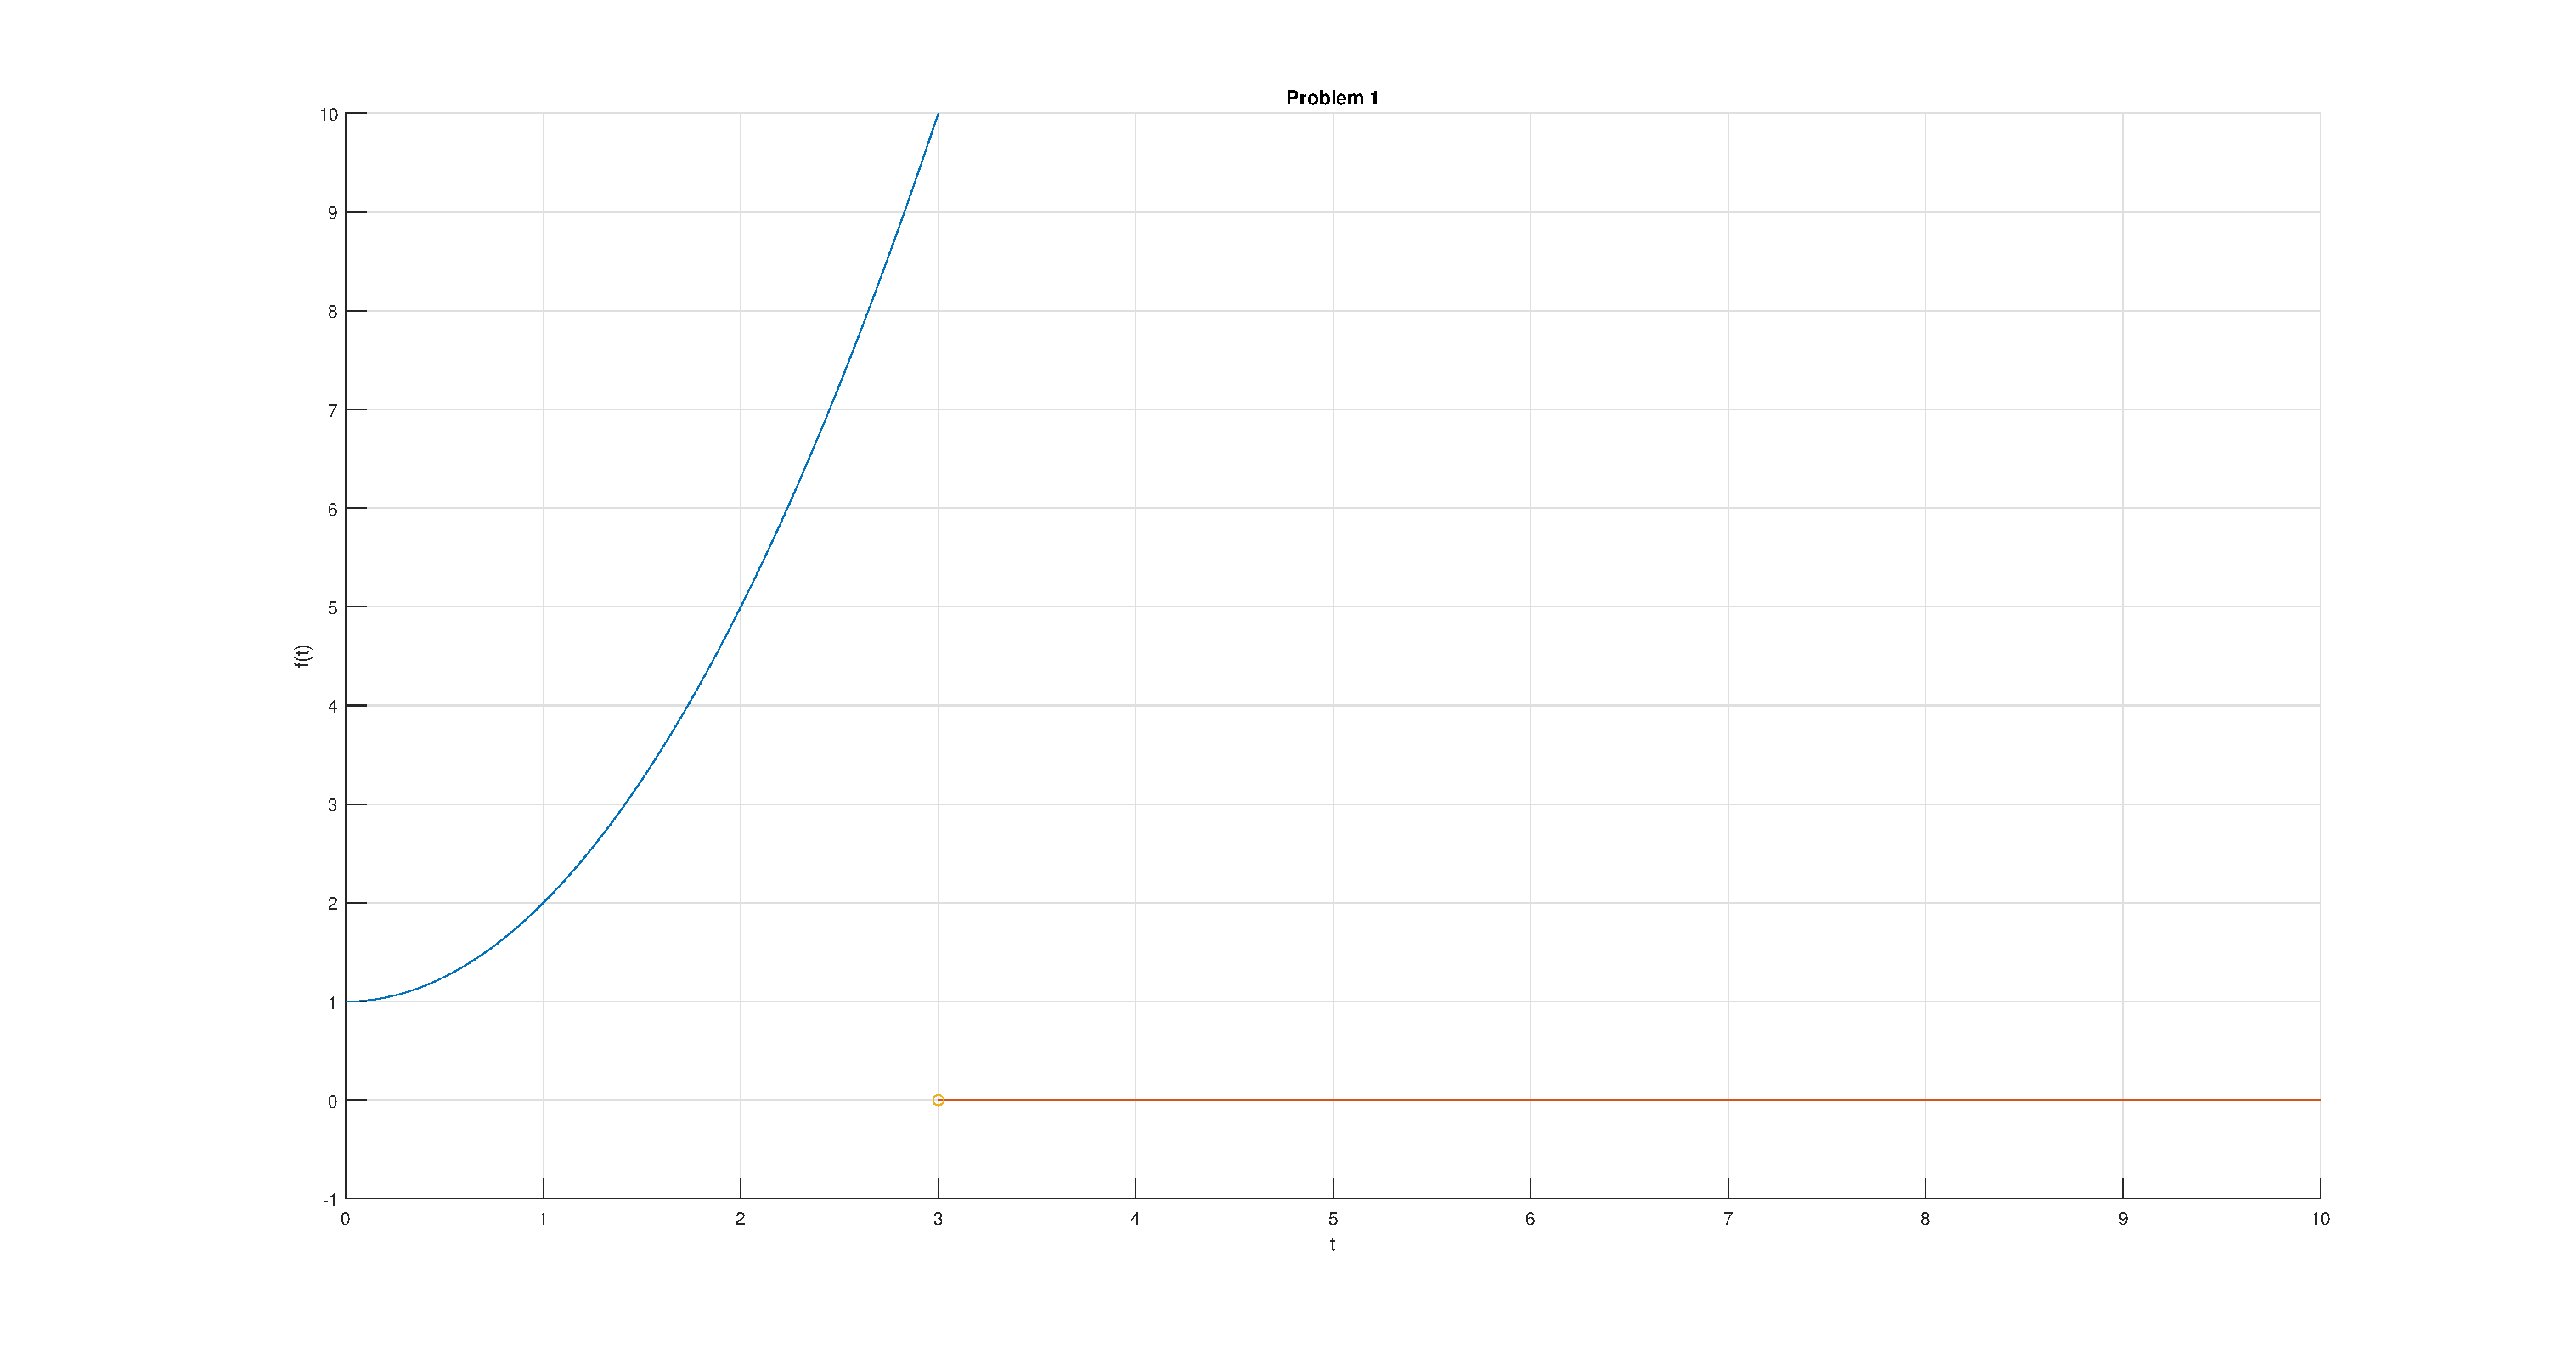
\includegraphics[width=16cm]{Prob1}
	\begin{align*}
		f(t) &= (t^2 + 1)(u_0(t) - u_3(t)) \\
		&= (t^2)u_0(t) + u_0(t) - ((t-3) + 3)^2u_3(t) - u_3(t) \\
		&= (t^2)u_0(t) + u_0(t) - (t-3)^2u_3(t) - 6(t-3)u_3(t) - 9u_3(t) - u_3(t) \\
		&= (t^2)u_0(t) + u_0(t) - (t-3)^2u_3(t) - 6(t-3)u_3(t) - 10u_3(t)
		\\ \\
		F(s) &= \frac{1}{s^2} + \frac{1}{s} - e^{-3s}\left(\frac{2}{s^3} + \frac{6}{s^2} + \frac{10}{s} \right)
	\end{align*}

\newpage

\noindent \textbf{Problem 2: }Solve the following initial value problem with Laplace transforms:
	$$
	y''  + 2y' + 5y = f(t) = 
	\begin{cases}
		5 & 0 \leq t \leq 4 \\
		-(t-9) & 4 \leq t \leq 9 \\
		0 & t > 9 
	\end{cases}, \qquad y(0) = 1, \qquad y'(0) = 4
	$$
Notice the following:
	\begin{align*}
		\mathcal{L}[y'' + 2y' + 5y] &= s^2Y(s) - sy(0) - y'(0) + 2sY(s) - 2y(0) + 5Y(s) \\
		&= (s^2 + 2s + 5)Y(s) - (s + 6) \\ \\ 
		f(t) &= 5(u_0(t) - u_4(t)) -(t-9)(u_4(t) - u_9(t)) \\
		&= 5u_0(t) - 5u_4(t) - ((t-4) - 5)u_4(t) + (t-9)u_9(t) \\
		&= 5u_0(t) - 5u_4(t) - (t-4)u_4(t) + 5u_4(t) + (t-9)u_9(t) \\
		&= 5u_0(t) - (t-4)u_4(t) + (t-9)u_9(t) \\
		\mathcal{L}[f(t)] &= \frac{5}{s} - \frac{e^{-4s}}{s^2} + \frac{e^{-9s}}{s^2}
	\end{align*}
Thus we get the equality:
	$$
	Y(s) = \frac{5}{s(s^2 + 2s + 5)} - \frac{e^{-4s}}{s^2(s^2 + 2s + 5)} + \frac{e^{-9s}}{s^2(s^2 + 2s + 5)} + \frac{s+6}{s^2 + 2s + 5}
	$$
Notice the partial fractions decomposition:
	\begin{align*}
		\frac{1}{s(s^2 + 2s + 5)} &= \frac{A}{s} + \frac{Bs + C}{s^2 + 2s + 5} \\
		1 &= (A+B)s^2 + (2A+C)s + 5A 
	\end{align*}
So we get $A = \frac{1}{5}, B = \frac{-1}{5}, C = \frac{-2}{5}$
	$$
	\frac{1}{s(s^2 + 2s + 5)} = \frac{1}{5s} - \frac{s + 2}{5(s^2 + 2s + 5)}
	$$
Notice the partial fractions decomposition:
	\begin{align*}
		\frac{1}{s^2(s^2 + 2s + 5)} &= \frac{A}{s} +  \frac{B}{s^2} + \frac{Cs + D}{s^2 + 2s + 5} \\
		1 &= (A+C)s^3 + (2A + B + D)s^2 + (5A + 2B)s + 5B
	\end{align*}
So we get $B = \frac{1}{5}, A = \frac{-2}{25}, C = \frac{2}{25}, \frac{-1}{25}$
	$$
	\frac{1}{s^2(s^2 + 2s + 5)} = \frac{-2}{25s} +  \frac{1}{5s^2} + \frac{2s - 1}{25(s^2 + 2s + 5)}
	$$
\newpage 

\noindent So we can now rewrite $Y(s)$
	\begin{align*}
		Y(s) &= \left(\frac{1}{s} - \frac{s + 1}{(s+1)^2 + 4} - \frac{1}{(s+1)^2 + 4} \right) - \frac{e^{-4s}}{25}\left(\frac{-2}{s} +  \frac{5}{s^2} + \frac{2(s+1)}{(s+1)^2 + 4} - \frac{3}{(s+1)^2 + 4}\right) \\
		 &+ \frac{e^{-9s}}{25}\left(\frac{-2}{s} +  \frac{5}{s^2} + \frac{2(s+1)}{(s+1)^2 + 4} - \frac{3}{(s+1)^2 + 4}\right) + \left(\frac{s+1}{(s+1)^2 + 4} + \frac{5}{(s+1)^2 + 4}\right)
	\end{align*}
Now we can take the Laplace inverse:
	\begin{align*}
		y(t) &= \left(1 - e^{-t}\cos(2t) - \frac{1}{2}e^{-t}\sin(2t) \right) - \frac{u_4(t)}{25}\left(-2 + 5(t-4) + 2e^{-(t-4)}\cos(2(t-4)) - \frac{3}{2}\sin(2(t-4)) \right) \\
		&+ \frac{u_9(t)}{25}\left(-2 + 5(t-9) + 2e^{-(t-9)}\cos(2(t-9)) - \frac{3}{2}\sin(2(t-9)) \right) + \left( \cos(2t) + \frac{5}{2} \sin(2t)\right)
	\end{align*}

\vspace{\baselineskip}
\vspace{\baselineskip}

\noindent \textbf{Problem 3: } The limiting solution is:
	\begin{align*}
		y(t) &= 1  - \frac{u_4(t)}{25}\left(-2 + 5(t-4) - \frac{3}{2}\sin(2(t-4)) \right) \\
		&+ \frac{u_9(t)}{25}\left(-2 + 5(t-9) - \frac{3}{2}\sin(2(t-9)) \right) + \left( \cos(2t) + \frac{5}{2} \sin(2t)\right)
	\end{align*}

\end{document}
